\documentclass {article}
\usepackage[margin=1 in]{geometry}
\usepackage{graphicx}
\usepackage{caption}
\usepackage{subcaption}
\usepackage{listings}
\begin{document}

\title {GPU correlator commissioning}
\author{Peeyush Prasad}
\maketitle

\section{Introduction}

The AARTFAAC 6-station  correlator is currently a GPU  based system developed by
John Romein. It is  implemented on AMD hardware, and is  based on a derivative of
the  Cobalt CPU  correlator  for LOFAR.  This  document describes  the data  and
control  flow from  the RSP  boards  to the  correlator output. It documents
the debugging of issues arising during the integration of the correlator into
the real-time pipeline,  and describes the scripts and tests developed during
this process. Some quirks of the system which might cause pitfalls during
further commissioning are  also documented.

\section {Data flow}
\textbf {Intra  station:}
\begin {itemize} 
  \item Each LBA antenna (consisting of two polarized outputs) of a station is
    connected  to an  RCU board,  which  carries out  analog conditioning  and
    sampling.  4  RCU boards are connected  to an RSP board,  which implements
    the PFB and subband selection for LOFAR.  These selected subbands are then
    beamformed in a regular LOFAR observation.  The station calibration tables
    are applied during beamforming. 12 RSP  boards are needed to handle the 48
    signal streams from the Dutch stations.

  \item Dipoles within a station are  connected to the digitizers (housed in a
    station cabinet) over 3 different  lengths of cable. A coarse compensation
    for the  delay differences in  the electrical  length of these  cables, as
    well as  their gain equalization is  applied by the RSP  boards. The above
    are common between LOFAR and AARTFAAC.

  \item The  AARTFAAC systen is independent  of LOFAR from this  stage, and is
    called  the  Subband  Data  Offload  (SDO)  interface.   AARTFAAC  has  an
    independent subband selection system, and  a copy of the selected subbands
    are forwarded for correlation and imaging.  Note that since these are raw,
    dipole level subbands, no station calibration has been applied on them.

  \item The  RSP boards generate a  copy of a  subset of the 512  subbands for
    AARTFAAC, and have special control  registers to configure AARTFAAC usage.
    These  additional subbands  are transmitted  over the  intra station  ring
    network,  but  via the  Uniboard-RSP  board  Interface (URI)  boards.   At
    present, the ring network bandwidth  allows 36 raw (unbeamformed) subbands
    of 16-bit  to be  transmitted from each  RSP board. This  can grow  to 72,
    8-bit and 144, 4-bit subbands, by setting  the bit mode. The URI boards (3
    per station, each  handling 4 RSP boards) reorganize the  data such that a
    subset of  subbands from its set  of 4 RSP  boards are routed on  a single
    data lane to  a uniboard Backnode (BN).   Thus, the 3 URI  boards route 36
    subbands from  all dipoles to  a single uniboard  BN, 9 subbands  per lane
    over 4 lanes.

  \item Each of  the 4 uniboard BNs  receives 9 subbands from  all dipoles. It
    selects 8 of the 9 subbands,  packetizes them by introducing a src/dest IP
    address and UDP  port. All BNs currently have the  same dest.  IP address,
    but with a different port number for different stations.

  \item  A pair  of BNs  send their  data over  the mesh  network to  a single
    FrontNode. The FN acts as a 10Gig  line handler, and transmits the data as
    UDP packets which contain 2 subbands. Thus, the packet rate from a station
    is half the rate of the subbands.

  \item  The  data  are  transmitted  over optical  fibre  to  Groningen.  The
    destination  IP address  and  port  number are  hardcoded  in the  station
    firmware, with  a board level DIP  switch to increment or  decrement these
    parameters. Thus, each station output  is a single 10GigE link, containing
    8 subbands from all 96 dipoles. All stations have the same IP address, but
    different UDP port numbers.\\
\end{itemize}

\textbf{Central Correlator  (Groningen):} At  Groningen, the 10GbE  data links
from  all stations  are  connected to  a  switch, which  has  a 40gbps  output
link. This  is connected to  a single GPU  based correlator machine,  which is
currently equipped  with a  Mellanox Technologies MT27500  Family [ConnectX-3]
Ethernet/Infiniband card, and a [AMD/ATI] Tahiti PRO GL [FirePro Series] GPU.

\section {Data Formats and Rates}
\subsection {Uniboard output (per station)}
The data packet  format of the frames generated by  the uniboard, and containing
all the station data is:
\begin{lstlisting}
typedef struct
{ unsigned int rsp_reserved_1:59
  unsigned int rsp_rsp_clock:1
  unsigned int rsp_sdo_mode:2
  unsigned int rsp_lane_id:2
  unsigned int rsp_station_id:16
  unsigned int nof_words_per_block:16  // 8sbbands X 96 dipoles=768 (4B = 1 word)
  unsigned int nof_blocks_per_packet:16 // 2
  unsigned int rsp_sync:1
  unsigned int rsp_reserved_0:13
  unsigned int rsp_bsn:50               // Two timeslices share the same BSN
} UniHdrType __aligned__(packed);

#define NRSUBBANDS 8
#define NRDIPOLES 96
typedef struct
{ short complex data [NRSUBBANDS][NRDIPOLES];
} RSPBlkType;

typedef struct
{ UniHdrType hdr;
  RSPBlkType blk[2]; // Two timeslices 
} UniUDPPktType;

\end{lstlisting}

Note that the lower timeslice is in  blk[0]. The number of data bytes in the UDP
payload  should  be:  2  (timesamples) * 8  (subbands) * 96  (dipoles)  *  4
(Bytes/sample) = 6144 bytes. The header is 22 bytes, resulting in a packet
size of 6166 Bytes at the correlator input.

\textbf {Data  rates} 200MHz sampling clock,  12 bit sampling per  dipole, PFB
applies a 1024 tap filter, resulting in subbands of 195312.5 Hz width.

The Uniboard packs 2 samples of each  subband from every dipole of the station
into  a single  packet, resulting  in a  packet rate  of ~100,000  packets per
second  from each  station  at the  Correlator. This  translates  to ~6166B  *
100,000,  or ~5  Gbps per  station, which  is sent  to the  GPU correlator  at
Groningen over a 10Gbps fibre link.

\subsection {Correlator output data  format} 
The datastream is  a linearized 4-D array, with dimensions  of time, baseline,
channel and  polarization.  Each  record has a  header with  meta information,
followed by  a blob  of visibilities. The  data can be  directed to  a network
port, or can be written to disk.  The header format is:
\begin{verbatim}
typedef  struct {
      uint32_t magic;
      uint32_t pad0;
      double   startTime, endTime;
      char     pad1[512 - 24];
    }HdrType;
\end{verbatim}
The block of size
\begin{verbatim}
unsigned nr_baselines = 288 * 289 / 2;
unsigned nr_channels = 63;
unsigned nr_polarizations = 4;

size_t block_size = header_size + sizeof(complex float) * nr_baselines *
nr_channels * nr_polarizations;
\end{verbatim}
can be read for a single timeslice. Within the blob, the pol. index moves the
fastest, followed by the channel, baseline and time indices.


\section {Timing Description}
\textbf {RSP board packet} Every RSP board  of a station is fed an aligned PPS
to mark absolute time. This is generated  at the center via a GPS, distributed
to stations over  the SyncOptics board, and aligned between  RSP boards by the
PAC board  (Confirm?). The RSP  board output  contains separate fields  in the
header relating to  the BSN and the  absolute timestamp. The BSN  is a counter
running on  the output  of the  1024 sample FFT  engine, i.e.,  BSNs increment
every 1024 samples of 160/200MHz. The BSN counter resets on the 1pps pulse.

Since  an   integer  number  of  blocks   does  not  exist  within   a  second
(195312.5/sec), the data is  split into an 'even' and an  'odd' second. In the
even second,  the BSN  max value  is 195312, while  in the  odd second,  it is
195313. Thus, absolute time  to the second can be read  off from the timestamp
field, while absolute time  within the second can be derived  in steps of 5.12
usec from the BSN number. 

\textbf  {Uniboard  packet} The  uniboard output  contains a
single, 50-bit  Block Sequence  Number (BSN) value  which serves as  an absolute
time in units of 5.12 usec. It is derived using the following formula from \cite{RP-1402}:
\begin{lstlisting}
BSN = (32b RSP timestamp * (RSP clock frequency/512) + g_adjust)/2 + 18b FSN
\end{lstlisting}
where the RSP timestamp is in seconds past 01Jan1970, g\_adjust is 1 for the even
seconds,  and  the  FSN  is  the  BSN  of the  RSP  board  (counter  running  at
1024/200MHz=5.12 usec intervals).



\section {Control flow}
\textbf {Station  level:} There are  96 RCUs corresponding  to the 2 pols  of 48
antennas. These are  connected to 12 RSP boards per station,  catering to 4 RCUs
of both pols per RSP board.  The RSPs are interconnected via a ring network. The
URI  boards tap  into the  ring network  to  move a  subset of  subbands to  the
uniboards.

The RSP control software (\verb+rspctl+ command  on the station LCUs) has been
augmented  to also  control AARTFAAC's  operation. This  option is  called the
Subband data output  (SDO) option.  The following options  are available (from
\verb+rspctl+ help):
\begin{verbatim}
--- Subband Data Output (SDO)
--------------------------------------------------------------------------------
rspctl --sdoenable[=0|1]                       # enable (or disable) sdo
output
rspctl --sdomode[=4|5|8|16]                    # set or get the number of bits
per sample
rspctl --sdo                 [--select=<set>]  # get sdo selection
rspctl --sdo=<set>           [--select=<set>]  # set sdo selection
\end{verbatim}

All  commands issued  without a  parameter report  their current  values.  The
sdomode command controls the bit mode  setting. This can be done independently
of LOFAR's  subband bitmode  setting. The  sdo command  shows which
subbands  are mapped  to  the 36  16-bit subbands  available  in the  RSPboard
output. This  is the entire  set of subbands  available to the  AARTFAAC. Note
that this  can be 72  subbands in  8-bit, and 144  subbands in 4-bit  mode.  A
sample output is:
\begin{verbatim}
RCU[ 0].subbands=1 x 36
[       590       592       594       596       598       600       602 
        604       606       608       610       612       614       616 
        618       620       622       624       626       628       630 
        632       634       636       638       640       642       644 
        646       648       650       652       654       656       658 
        660 ]

RCU[ 1].subbands=1 x 36
[       591       593       595       597       599       601       603 
        605       607       609       611       613       615       617 
        619       621       623       625       627       629       631 
        633       635       637       639       641       643       645 
        647       649       651       653       655       657       659 
        661 ]
<snip>
...
RCU[95].subbands=1 x 36
\end{verbatim}
This shows the subband numbers (between 0-511) routed to AARTFAAC. Here, the X and Y
pols  occupy consecutive  subband numbers.  Since consecutively  numbered RCUs
serve  X and  Y pols,  consecutive subband  numbers are  seen spread  over two
consecutive RCUs. Hence, subband 591 corresponds to (591-1)/2 =subband 295 of
the Y pol.\\

\textbf {AARTFAAC specific station hardware:}  A control machine for controlling  the uniboards is
available   (lcu-aartfaac.control.lofar   (10.151.252.190),  accessible   from
<username>@portal.lofar.eu)  The  uniboards  can   be  treated  as  unilateral
transmitters,  although Rx  and  Tx  packet counters  can  be  read off  their
registers,  and can  be used  to monitor  the board.   This becomes  important
because the  Uniboard FPGAs have a  factory image loaded on  poweron, with the
requirement of explicitly  loading the AARTFAAC image. Details  on the control
of AARTFAAC uniboards is available in \cite{RP-1463}.

\textbf {GPU Correlator:} The correlator machine is currently gpu02.das4.astron.nl,
and is a part  of the DAS4 cluster.  It will ultimately  be moved to a dedicated
machine with twin  GPUS. The correlator sources and binaries  are located in the
~romein/projects/Triple-A/AARTFAAC folder.  The file hierarchy is expected to be
maintained in  the production  machine.\\ The correlator  top level  source (and
binary) are called  'AARTFAAC'.\\ A convenient script called  'run' is available
to  run  the  correlator with  default  options,  while  routing the  output  to
file. The  available options (and  their default values in the run script) are:
\begin{verbatim}
DISPLAY=:0 PLATFORM="AMD Accelerated Parallel Processing" TYPE=GPU numactl -C 11-19 ~romein/projects/Triple-A/AARTFAAC/AARTFAAC -p1 -n288 -t3072 -c64 -d0 -g0 -b16 -s8 -R1 -r720 -i 10.99.100.1:53268,10.99.100.1:53276,10.99.100.1:53284,10.99.100.1:53292,10.99.100.1:53300,10.99.100.1:53308 -o file:sb0,null:,null:,null:,null:,null:,null:,null: "$@" 2>&1 | tee sb0.log

-p1    = Turn on/off profiling
-n288  = Number of stations
-t3072 = Number of samples per channel.
-c64   = Number of channels per subband.
-d0    = Turn on/off delay compensation
-g0    = set GPUs (?)
-b16   = bit mode of incoming data (bits/sample)
-s8    = Number of input subbands
-R1    = Turn on Realtime processing
-r30   = Integration time (?)
-i
10.99.100.1:53268,10.99.100.1:53276,10.99.100.1:53284,10.99.100.1:53292,10.99.100.1:53300,10.99.100.1:53308
= IP address and port numbers of the incoming subbanded data per station.
-o file:/tmp/sb2,null:,null:,null:,null:,null:,null:,null: = output location for the 8 correlated subbands. The above string indicates that only sb0 is written to disk. 


To route the correlator output over the network to TCP port 20000 on ais001:
-o tcp:10.144.6.13:20000,null:,null:,null:,null:,null:,null:,null:


Other interesting options are:
-a1    = Turn on/off subband bandpass correction after channelization
-I     = Visibility integration (?)
-P2    = Number of polarizations
-S4    = Number of generated stokes(?)
\end{verbatim}

\section {Correlator debugging}


\section {Helper programs}
All helper programs (as well as the latest copy of this document) are
available on github:afaac_GPU_corr/src. The Uniboard_FP7 scripts are available
on svn at https://svn.astron.nl/UniBoard_FP7/Aartfaac/trunk/Software/python/apps/aartfaac_sdo/

\begin {itemize}
  \item check_stations.sh: Bash script to dump packets from the 40Gbps
    interface on the GPU machine, a crude check on whether stations are
    sending data.\\ NOTE: A better check is the eth2_packet_rate.py program,
    which calculates the rate of incoming packets. If all stations are sending
    data, the received data rate on the GPU machine should be ~29 Gbps.

  \item \textbf{Raw data dump to disk:} Use udp-copy.c (author John Romein). A
    snapshot of this is available within teh afaac_GPU_corr repository.
  
  \item udp_copy_stations.sh: Script which uses udp-copy underneath. Creates
    raw (uniboard) data files corresponding to each station in /tmp (which is
    an SSD) with an appropriate local timestamp.

  \item showvisrawtime.c: Prints out the timestamps in unix time for the
    binary visibilities written to disk by the correlator. To convert to time
    in the current timezone, use the command date -d @<timeoutput as unixtime> 

  \item gpu2mat.py: convert the full-pol, 63 channel visibility data generated
    by the GPU correlator into a .mat file of visibilities.

  \item showgpuacm.m: Matlab script to take the output of gpu2mat.py and
    display the covariance matrix of each integration time on an updating figure.

  \item rsp2gpu.c: Converts dipole level subbanded data as recorded by LOFAR
    infrastructure during earlier AARTFAAC trial observations into 

  \item  run.off.[del|nodel]: Script to run the correlator in offline mode, on the
    output of udp_copy_stations.sh. Takes the timestamp as a command line
    input. Separate scripts for applying offline inter station delay
    correction via phase ramps.

  \item run.rt.[del|nodel]: Similar to above, but in real-time mode.

  \item run.rt.nodel.ais: Similar to above, but now writing out visibility
    data to the ais001.control.lofar machine.

\end{itemize}

\section {Data}
Data was recorded from the GPU correlator, with the output being written to
disk. The helper program showrawtime.c extracts out just the timestamp from
large datasets to determine if any time samples are missed. (Who generates the
timestamps?). 


The script gpu2mat.py converts the incoming data to a 4D complex array with dimensions
of time, bline, chan, pol, and writes it as a .mat file. The script
showgpuacm.m can be used to display the received ACMs.


\begin{figure*}[tbh]
 \center{
        {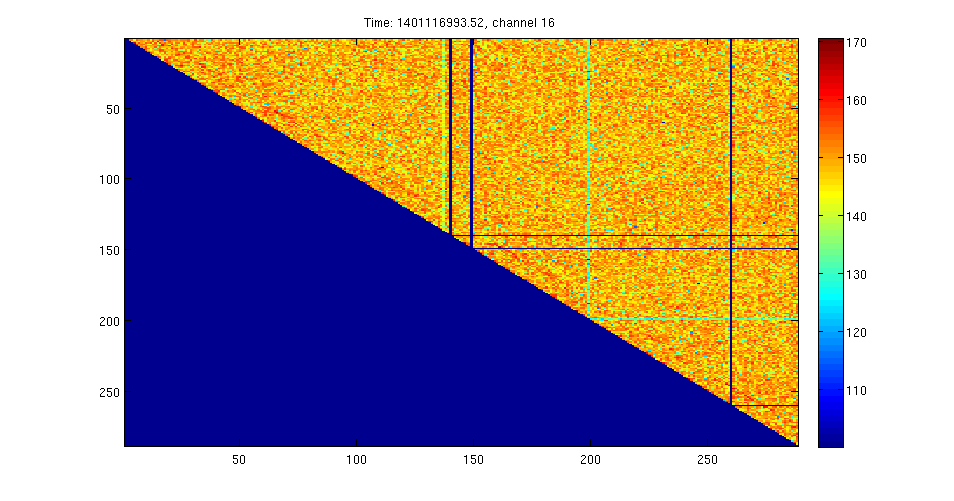
\includegraphics[width=0.8\textwidth] {Figs/sb0_acm.png}}
        {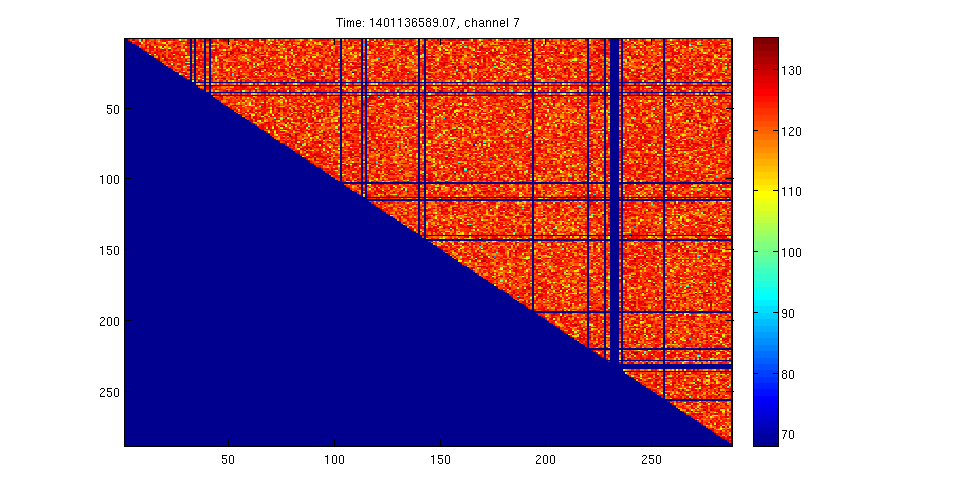
\includegraphics[width=0.8\textwidth] {Figs/sb1_acm.png}}
        {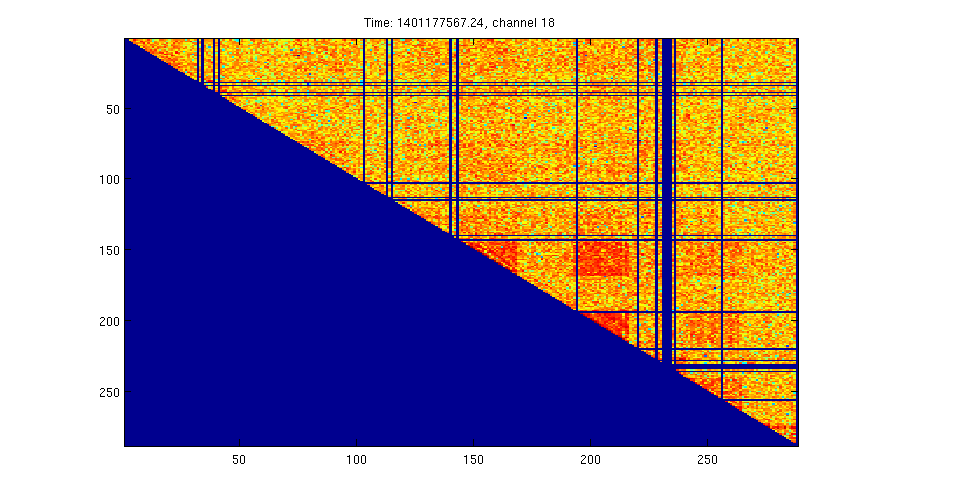
\includegraphics[width=0.8\textwidth] {Figs/sb2_acm.png}}
 \caption{Snapshot Covariance matrices from subband 0, 1, 2. Visibility powers
   in dB, recorded on 26,27May14}
 \label {inner_outer_uvcov}
 }
\end{figure*}

\begin{figure*}[tbh]
 \center{
        {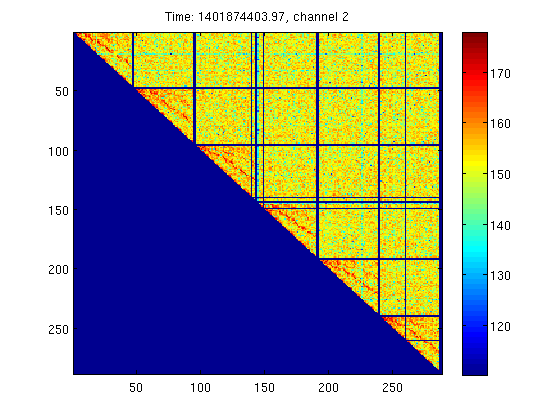
\includegraphics[width=0.8\textwidth] {Figs/sb0_04Jun14.png}}
 \caption{Snapshot Covariance matrices from  subband 0. Visibility powers in dB,
   recorded on 04Jun14.  The missing last two dipoles from  each station seem to
   indicate this being an LBA\_INNER observation. }
 \label {inner_outer_uvcov}
 }
\end{figure*}



\section {gpu2mat.py}
\begin{verbatim}
#!/usr/bin/python
# Program to extract visibility data from the AARTFAAC GPU correlator output
# stream, and write out a .mat file.
# pep/03Jun14

import sys;
import traceback
import numpy;
import os;
import struct;
import scipy.io as sio;

def main ():
	if (len(sys.argv) < 2):
		print 'Usage: ', sys.argv[0], ' rawfile.dat';
		print '       Converts correlated output as generated by AARTFAAC GPU correlator';
		print '       into a .mat file.\n';
		sys.exit (-1);

	nelem  = 288;       
	nrec = 10;
	nbline= nelem*(nelem+1)/2; 
	nchan = 63;
	npol = 4;

	hdrsize = 512;
	recsize = hdrsize + nbline*nchan*npol*2*4; # 4 is for sizeof (float), 2 is for complex float.

	
	# Create an array for every timeslice from all subbands
	tobs = numpy.zeros (nrec, 'd'); # Time of obs, as double
	acm = numpy.zeros ([nrec, nbline, nchan, npol, 2], 'f');
	
	# Output .mat file
#	foutname = sys.argv[1].split('.')[0] + '.mat';
#	print 'Writing to file: ', foutname;
#	if not os.path.isfile (foutname):
#		ffloat = open (foutname, 'wb');
#	else:
#		print '	   ### File exists! Quitting!';
#		sys.exit (-1);
	
	print 'Operating  with : %d pols, %d chans, %d blines' %(npol, nchan, nbline);
	print 'Header/rec size : %d/%d bytes' % (hdrsize, recsize);
	print 'Records per file: %d' % nrec;
	# open file
	fin = open (sys.argv[1], "rb");
	ind = 0;
	doneRead = 0;
	while doneRead == 0:
		for ind in range (0, nrec):
			# Read in record from file
			rec = fin.read(recsize);
			if not rec: 
				print 'EOF reached. Last few records may be discarded.\n';
		 		doneRead = 1; break;
	
			(magic, pad0, startTime, endTime) = struct.unpack ("<IIdd", rec[0:24]);
			print 'Start: %.2f, End: %.2f' % (startTime, endTime);
			tmp = numpy.reshape (numpy.asarray (struct.unpack ("ff"*nbline*nchan*npol, rec[512:])),[nbline, nchan, npol, 2]);
			acm [ind] = tmp;
			tobs[ind] = startTime;
			# print 'Type of acm' , type(acm);
			# print 'Shape of array: ', acm.shape;
	
		fname = '%s_%d-%d.mat'%(sys.argv[1], tobs[0], tobs[nrec-1]);
		print 'Writing to file %s.\n' % fname;
		sio.savemat (fname, {'acm':acm, 'tobs':tobs});

	# ffloat.close ();
	fin.close ();
	return;

if __name__ == "__main__":
	main ();
\end{verbatim}

\begin{thebibliography}{1}

\bibitem {RP-1402} LOFAR RSP – SDO Interface Specification, ASTRON-RP-1402

\bibitem {RP-1403} UniBoard – UDP – SDO Interface Specification,
  ASTRON-RP-1403
\bibitem {RP-1462} AARTFAAC Subband data offload manual, ASTRON RP-1462

\end{thebibliography}
\end{document}
